\documentclass[a0,final]{a0poster}
%%%Load packages
\usepackage{multicol} 			%3-column layout
\usepackage[left=2cm,right=2cm,bottom=0cm,top=0cm]{geometry}			%Reset margins
\usepackage{mathpazo}			%Load palatino font & pazo math
\usepackage{color}				%Needed for colour boxes & coloured text
\usepackage{graphics}
\usepackage[export]{adjustbox}
\usepackage{url}
\usepackage{mathtools}
\usepackage{amsmath}
\usepackage{amsfonts}
\usepackage{amssymb}
\usepackage{graphicx}
\usepackage{float}
\usepackage{booktabs}
\usepackage{caption}
\usepackage{subcaption}
\usepackage{booktabs}
%\usepackage{dblfnote}

%%%Define colours and lengths
\definecolor{headingcol}{rgb}{1,1,1}			%Colour of main title
\definecolor{boxcol}{rgb}{0.7,0.3,0.2}		%Edge-colour of box and top banner
\fboxsep=1cm							%Padding between box and text
\setlength{\columnsep}{2cm}				%Set spacing between columns
\renewcommand{\familydefault}{\sfdefault}	%Set main text to sans-serif

%%%Format title
\makeatletter							%Needed to include code in main file
\renewcommand\@maketitle{%
\null									%Sets position marker
{
\color{headingcol}\sffamily\Huge		%Set title font and colour
\@title \par}%
\vskip 0.6em%
{
\color{white}\sffamily\large				%Set author font and colour
\lineskip .5em%
\begin{tabular}[t]{l}%
\@author
\end{tabular}\par}%
\vskip 1cm
\par
}
\makeatother

\title{Modeling and Simulating Political Violence\\and Optimizing Aid Distribution in Uganda}

\author{Peter Bull \& Isaac Slavitt\\
Harvard University - AM207}

\begin{document}


\hspace{-3cm}								%Align with edge of page, not margin
\colorbox{boxcol}{						%Coloured banner across top
%\begin{minipage}{1189mm}					%Minipage for title contents
\begin{minipage}{600mm}
\maketitle
\end{minipage}
\begin{minipage}{575mm}					%Minipage for title contents

\includegraphics[width=1\textwidth,right]{iacs_logo.png}
\end{minipage}}

\vspace{1cm}

\begin{multicols}{3}							%Use 3-column layout
\raggedcolumns							%Don't stretch contents vertically

%%%Column1
\section*{Overview}

\vspace{-6mm}

Using MCMC techniques, we model civil conflict in Uganda and optimize the limited relief aid that can be provided in these scenarios. We describe a method to simulate civil conflict events in space and time given historical data about these events. We also optimize the distribution of limited aid resources to refugees from these crises. Modeling aid delivery as a combination of the traveling salesman problem and the knapsack algorithm --- two NP-hard problems --- we find acceptable solutions using stochastic metaheuristics.\\

\vspace{-5mm}

\begin{figure}[H]
\centering
  \begin{subfigure}[b]{0.48\columnwidth}
    \centering
    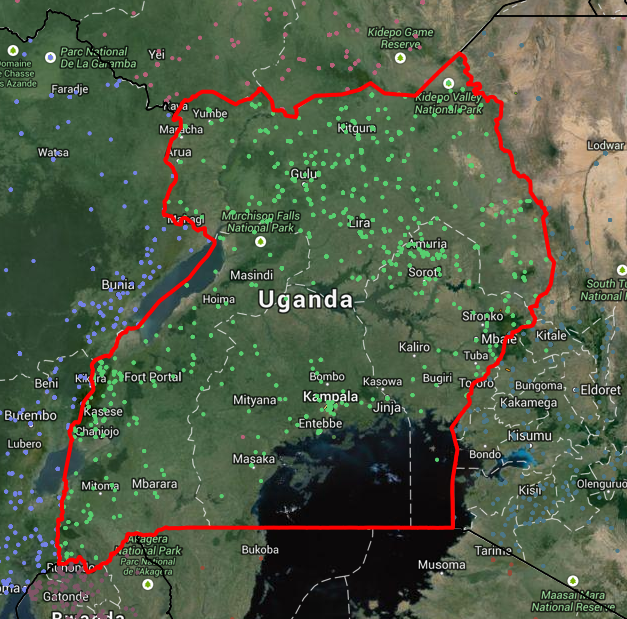
\includegraphics[width=\textwidth]{../write-up/figures/uganda}
    \caption{Scatterplot of conflicts.}
    \label{fig:map-points}
  \end{subfigure}~\begin{subfigure}[b]{0.49\columnwidth}
    \centering
    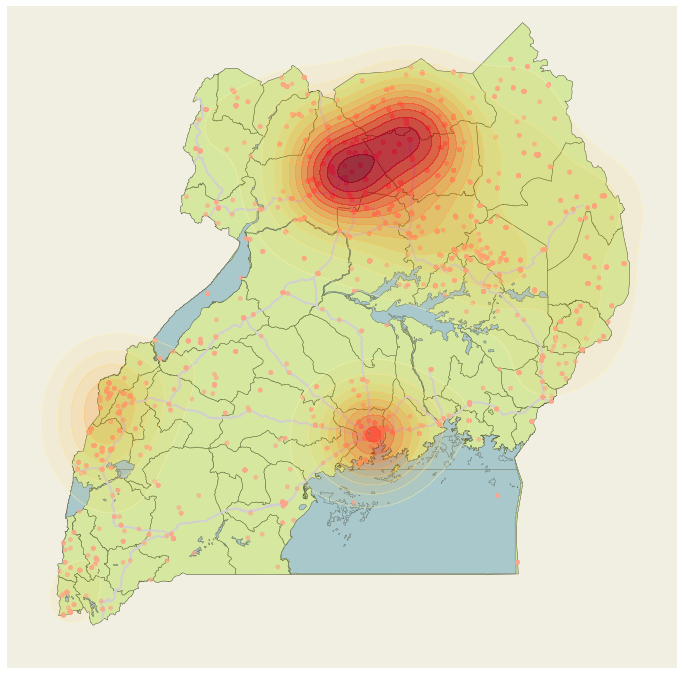
\includegraphics[width=\textwidth]{../write-up/figures/map-with-smoothed-data}
    \caption{Mat\'{e}rn smoothed.}
    \label{fig:map-smooth}
  \end{subfigure}
  \caption{Civil conflicts in Uganda 1997-2013.}
  \label{fig:map}
\end{figure}

\noindent The data comes from ACLED (Armed Conflict Location and Event Data Project), which is a dataset with locations, dates, fatalities, motivation, actors involved, and other information about civil conflicts in Africa. Their collection of data on Uganda covers 1997-2013, and they have a real-time tracker of events reported in 2014.\cite{ACLED}

\vspace{-6mm}

\section*{Modeling events in space}

\vspace{-6mm}

We treat the entire country of Uganda as a probability distribution from which geospatial conflict events could be sampled.  We took historical conflict location data from the entire ACLED data set and smoothed it using a Mat\'{e}rn covariance function.  Figure \ref{fig:map-smooth} shows this smoothing applied to the same conflicts depicted in \ref{fig:map-points}. This estimate (i.e., the empirical distribution of the conflict data), has a complex functional form which makes it challenging to sample from. However, it is simple for a given coordinate to get the probability of an event. Given this property of our smooth, we can apply MCMC sampling techniques to generate samples from this probability distribution. Figure \ref{fig:histogram} shows the distribution of the samples as a two-dimensional histogram.

\begin{figure}[H]
  \centering
  \begin{subfigure}[b]{0.5\columnwidth}
    \centering
    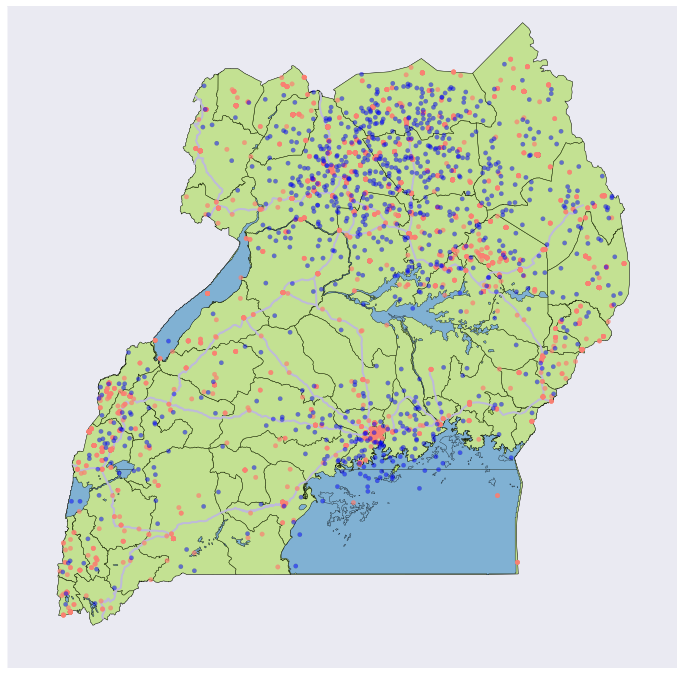
\includegraphics[width=\textwidth]{../write-up/figures/1000-slice-samples}
    \caption{Blue dots are samples from the empirical distribution.}
    \label{fig:sampled-conflicts}
  \end{subfigure}~\begin{subfigure}[b]{0.5\columnwidth}
    \centering
    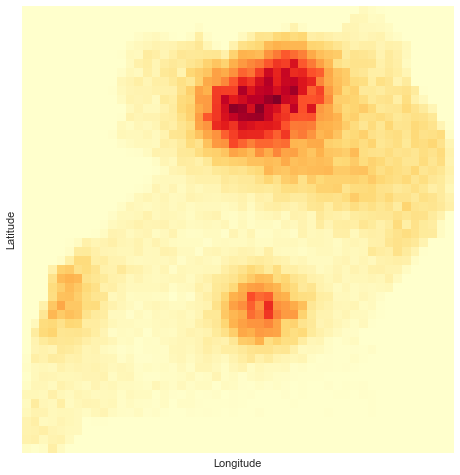
\includegraphics[width=\textwidth]{../write-up/figures/histogram}
    \caption{2D histogram of slice samples from the empirical distribution.}
    \label{fig:histogram}
  \end{subfigure}
  \caption{Discretizing and sampling from the conflict distribution.}
\end{figure}

\columnbreak
%%%%%%%%%%%%%%%%%%%%%%%%%%%%%%%%%%%%%%%%%%%%%%%%%%%%%%%%%%%%%%%%%%%%%%%%%%%%
%%%Column 2

\vspace{-10mm}

\section*{Modeling events in time}

\vspace{-6mm}

To model events in time, we use an autoregressive Poisson GLM. The Poisson GLM lets us have a linear relation between previous data and the mean of a Poisson distribution. This will allow us to retain the probabilistic interpretation of the events in time.

\begin{figure}[H]
\centering
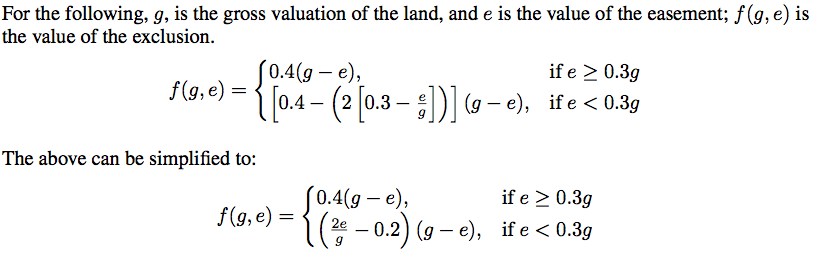
\includegraphics[scale=1]{../write-up/figures/poisson-regression.png}
\caption{Poisson regression.}
\label{fig:poisson}
\end{figure}

\noindent In order to model events using a Poisson distribution, we must discretize our time dimension. We opted for month-long increments. The thinking behind this decision is that we want to use sample draws to run our aid optimizations. If a model like this were to be used in planning for future conflicts, having a month-long window for a plan seems like a good balance between precision and logistic concerns.

\section*{Optimizing Aid Delivery}

\vspace{-6mm}

\subsection*{The Traveling Salesman Problem}

\vspace{-6mm}

Let's postulate a Red Cross medical or food supply caravan that originates from the organization's in-country headquarters. This caravan wishes to visit all $n$ emergent locations in order to deliver needed supplies in the most efficient manner possible. Here is the traditional convex optimization specification of the problem:\cite{Winston}

\vspace{-10mm}

\begin{align*}
\min &\sum_{i=0}^n \sum_{j\ne i,j=0}^nc_{ij}x_{ij} &&  \\
\mathrm{s.t.} \; \; & x_{ij} \in \{0, 1\} && i,j=0, \cdots, n \\
	& \sum_{i=0,i\ne j}^n x_{ij} = 1 && j=0, \cdots, n \\
	& \sum_{j=0,j\ne i}^n x_{ij} = 1 && i=0, \cdots, n \\
	&u_i-u_j +nx_{ij} \le n-1 && 1 \le i \ne j \le n
\end{align*}

\noindent Where $x_{ij}$ is a binary decision variable indicating whether we go from location $i$ to location $j$, $c_{ij}$ is the distance between location $i$ and location $j$, the objective function is the sum of the distances for routes that we decide to take, and the final constraint ensures that all locations are visited once and only once.


\begin{figure}[H]
  \centering
  \begin{subfigure}[b]{0.5\columnwidth}
    \centering
    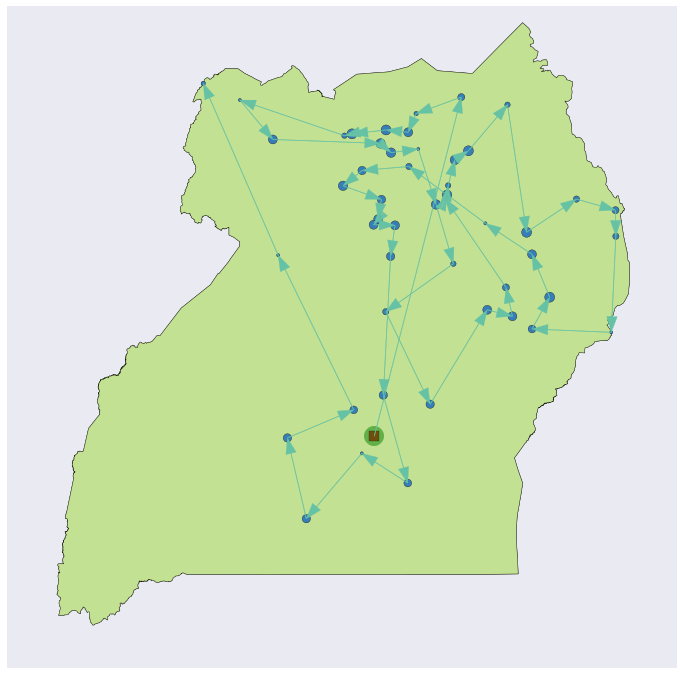
\includegraphics[width=\textwidth]{../write-up/figures/routing-vanilla-tsp}
    \caption{Visiting all cities without reloading.}
    \label{fig:routing-vanilla-tsp}
  \end{subfigure}~\begin{subfigure}[b]{0.5\columnwidth}
    \centering
    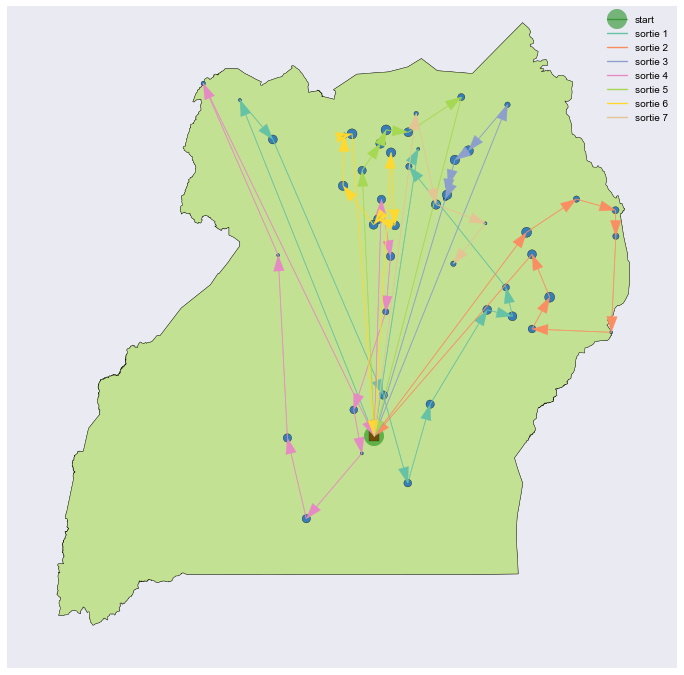
\includegraphics[width=\textwidth]{../write-up/figures/routing-reloading}
    \caption{Routing with reloading HQ in capital city Kampala.}
    \label{fig:routing-reloading}
  \end{subfigure}
  \caption{Optimizing aid delivery routing using one random sample of conflicts.}
\end{figure}

\columnbreak


%%%%%%%%%%%%%%%%%%%%%%%%%%%%%%%%%%%%%%%%%%%%%%%%%%%%%%%%%%%%%%%%%%%%%%%%%%%%
%%%Column 3

\subsection*{Packing the aid truck --- adding in Knapsack Problem}

\vspace{-6mm}

We extend the TSP into a multi-objective optimization problem
where \textbf{the contents of the aid trucks} also have an optimization component. In the real world, we can't pack unlimited supplies for an aid delivery trip. Therein lies
the knapsack problem: subject to a volume or weight constraint, and given that different locations
might have very different needs such as food, vaccinations, or emergent medical supplies, \textbf{which supplies do we pack on the trucks}?  Often, this problem is formulated such that you can only bring one of each item, but that doesn't make sense here. We want to be able to bring as many types of each type of aid as we think necessary, and we'll assume that as many as desired are available to load on the trucks before starting out from HQ. Here's the unbounded version of the knapsack problem:

\begin{align*}
\max &\sum_{i=1}^n v_i x_i &&  \\
\mathrm{s.t.} \; \; & x_i \in \mathbb{Z}, \; x_i \geq 0 \; \sum_{i=1}^n w_ix_i \leq W
\end{align*}

\noindent In this formulation, $x_{i}$ is a zero or positive integer decision variable indicating how many units of item $i$ we load on the truck, $v_i$ is the utility we get from bringing along item $i$, $w_i$ is the weight of item $i$, $W$ is the maximum that can be loaded. We use simulated annealing (SA) to get acceptable solutions to the TSP. The SA algorithm is minimizing is a \textbf{loss function} that heavily penalizes running short of supplies. Figure \ref{fig:routing-reloading} shows this problem integrated with the TSP.

\vspace{-6mm}

\begin{figure}[H]
  \centering
  \begin{subfigure}[b]{0.5\columnwidth}
    \centering
    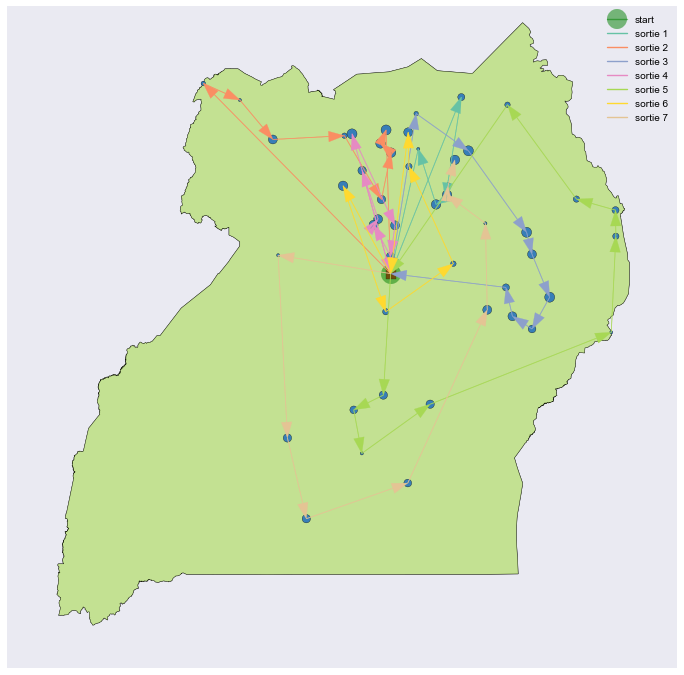
\includegraphics[width=\textwidth]{../write-up/figures/routing-reloading-hq-optimal}
    \caption{Routing with reloading from optimal HQ.}
    \label{fig:routing-reloading-hq-optimal}
  \end{subfigure}~\begin{subfigure}[b]{0.5\columnwidth}
    \centering
    \centering
    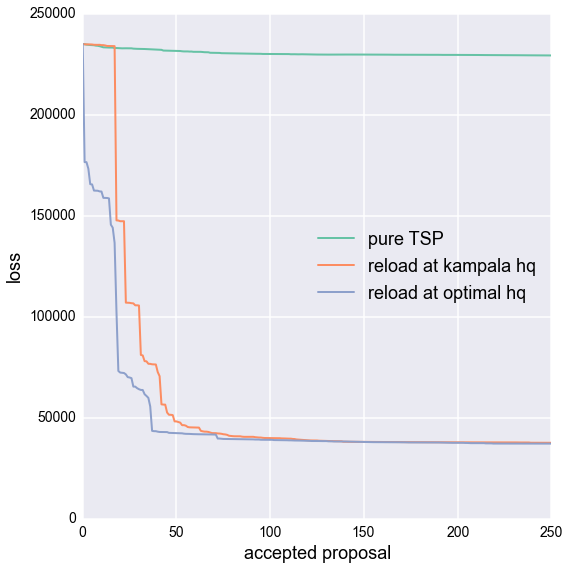
\includegraphics[width=\textwidth]{../write-up/figures/comparative-loss-plot}
    \caption{Example loss function optimization convergence for $n=50$.}
    \label{fig:comparative-loss-plot}
  \end{subfigure}
  \caption{Optimizing aid delivery routing with reloading.}
\end{figure}

\vspace{-15mm}

\subsection*{Locating HQ optimally for efficient reloading}

\vspace{-6mm}

Although we have now optimized our route so that we never run out of supplies, we should ask whether our HQ could be more conveniently located. We can answer this by treating the reload location as another set of parameters and continuing to sample HQ locations using SA. Figure \ref{fig:routing-reloading-hq-optimal} shows the TSP/Knapsack optimized once again, this time using a the optimal HQ location, while \ref{fig:comparative-loss-plot} compares the loss function as each method converges to its best possible configuration.

\vspace{-6mm}

\section*{Conclusions}

\vspace{-6mm}

In each part of this problem, analytical solutions either do not exist (e.g. in simulation) or are computationally infeasible (e.g. in the TSP/Knapsack optimizations).  We found that using a metaheuristic such as SA converged on robust solutions in relatively short order.  Future research might include adding many more constraints or twists to the problem, and trying different stochastic optimization techniques such as genetic optimization, Tabu search, or ant colony optimization.

\vspace{-6mm}

\bibliographystyle{ieeetr}
\bibliography{poster}

\end{multicols}
\end{document}
